\documentclass[11pt]{article}
\usepackage{amsfonts}
\usepackage{amsmath}
\usepackage{booktabs}
\usepackage{caption}
\usepackage[sort,nocompress]{cite}
\usepackage{color}
\usepackage{enumitem}
\usepackage{fancyhdr}
\usepackage{hyperref}
\usepackage{lastpage}
\usepackage{pgfplots}
\usepackage{rotating}
\usepackage{siunitx}
\usepackage{subfigure}
\usepackage{tikz}
\usepackage{tikz-3dplot}
\usepackage{titlesec}
\usepackage{todonotes}
\usepackage{wrapfig}
\usepackage{verbatim}
%\usepackage{showkeys}

\usetikzlibrary{shapes,arrows}

\addtolength{\oddsidemargin}{-0.75in}
\addtolength{\evensidemargin}{-0.75in}
\addtolength{\textwidth}{1.5in}
\addtolength{\topmargin}{-0.75in}
\addtolength{\textheight}{1.5in}
% For 11pt size

\titleformat*{\section}{\large\bfseries}
\titleformat*{\subsection}{\normalsize\bfseries}

\newcommand{\bd}{\partial}
\newcommand{\BL}{\mathrm{BL}}
\newcommand{\bigO}{\mathcal{O}}
\newcommand{\cc}{\mathbf{c}}
\newcommand{\dlp}{{\mathrm{dlp}}}
\newcommand{\ee}{\mathbf{e}}
\newcommand{\ff}{\mathbf{f}}
\newcommand{\FF}{\mathbf{F}}
\renewcommand{\gg}{\mathbf{g}}
\newcommand{\II}{\mathcal{I}}
\newcommand{\mcaption}[2]{\caption{\small \em #1}\label{#2}}
\newcommand{\nn}{\mathbf{n}}
\newcommand{\NN}{{\mathbf{N}}}
\newcommand{\pderiv}[2]{\frac{\partial #1}{\partial #2}}
\newcommand{\pderivtwo}[2]{\frac{\partial^{2} #1}{\partial #2^{2}}}
\newcommand{\pphi}{{\boldsymbol{\phi}}}
\renewcommand{\Re}{{\textrm{Re}}}
\newcommand{\rr}{{\mathbf{r}}}
\newcommand{\RR}{{\mathbb{R}}}
\newcommand{\slp}{{\mathrm{slp}}}
\newcommand{\ssigma}{{\boldsymbol{\sigma}}}
\newcommand{\SLP}{{\mathtt{SLP}}}
\newcommand{\DD}{{\mathcal{D}}}
\renewcommand{\SS}{{\mathcal{S}}}
\newcommand{\ttau}{{\boldsymbol{\tau}}}
\newcommand{\uu}{\mathbf{u}}
\newcommand{\vv}{\mathbf{v}}
\newcommand{\VV}{{\mathcal{V}}}
\newcommand{\xx}{\mathbf{x}}
\newcommand{\yy}{\mathbf{y}}
\newcommand{\thL}{$\theta$--$L$}

\pagestyle{fancy}
\lhead{\footnotesize Bryan Quaife}
\chead{\footnotesize Viscous Erosion of a Porous Medium}
\rhead{\footnotesize \thepage}
\cfoot{}

%\usepgfplotslibrary{external}
%\tikzexternalize



\begin{document}
\begin{center}
Viscous Erosion of a Porous Medium \\
Bryan Quaife, Assistant Professor \\
Florida State University \\
512-436-1148, bquaife@fsu.edu \\
DOE/Office of Science Program Office: ASCR-Applied Mathematics \\
Funding Opportunity Announcement Number: DE-FOA-0001968
\end{center}

%%%%%%%%%%%%%%%%%%%%%%%%%%%%%%%%%%%%%%%%%%%%%%%%%%%%%%%%%%%%%%%%%%%%%%%%%%%%%
\section{Introduction}
\begin{wrapfigure}[22]{r}{0.6\textwidth}
\centering
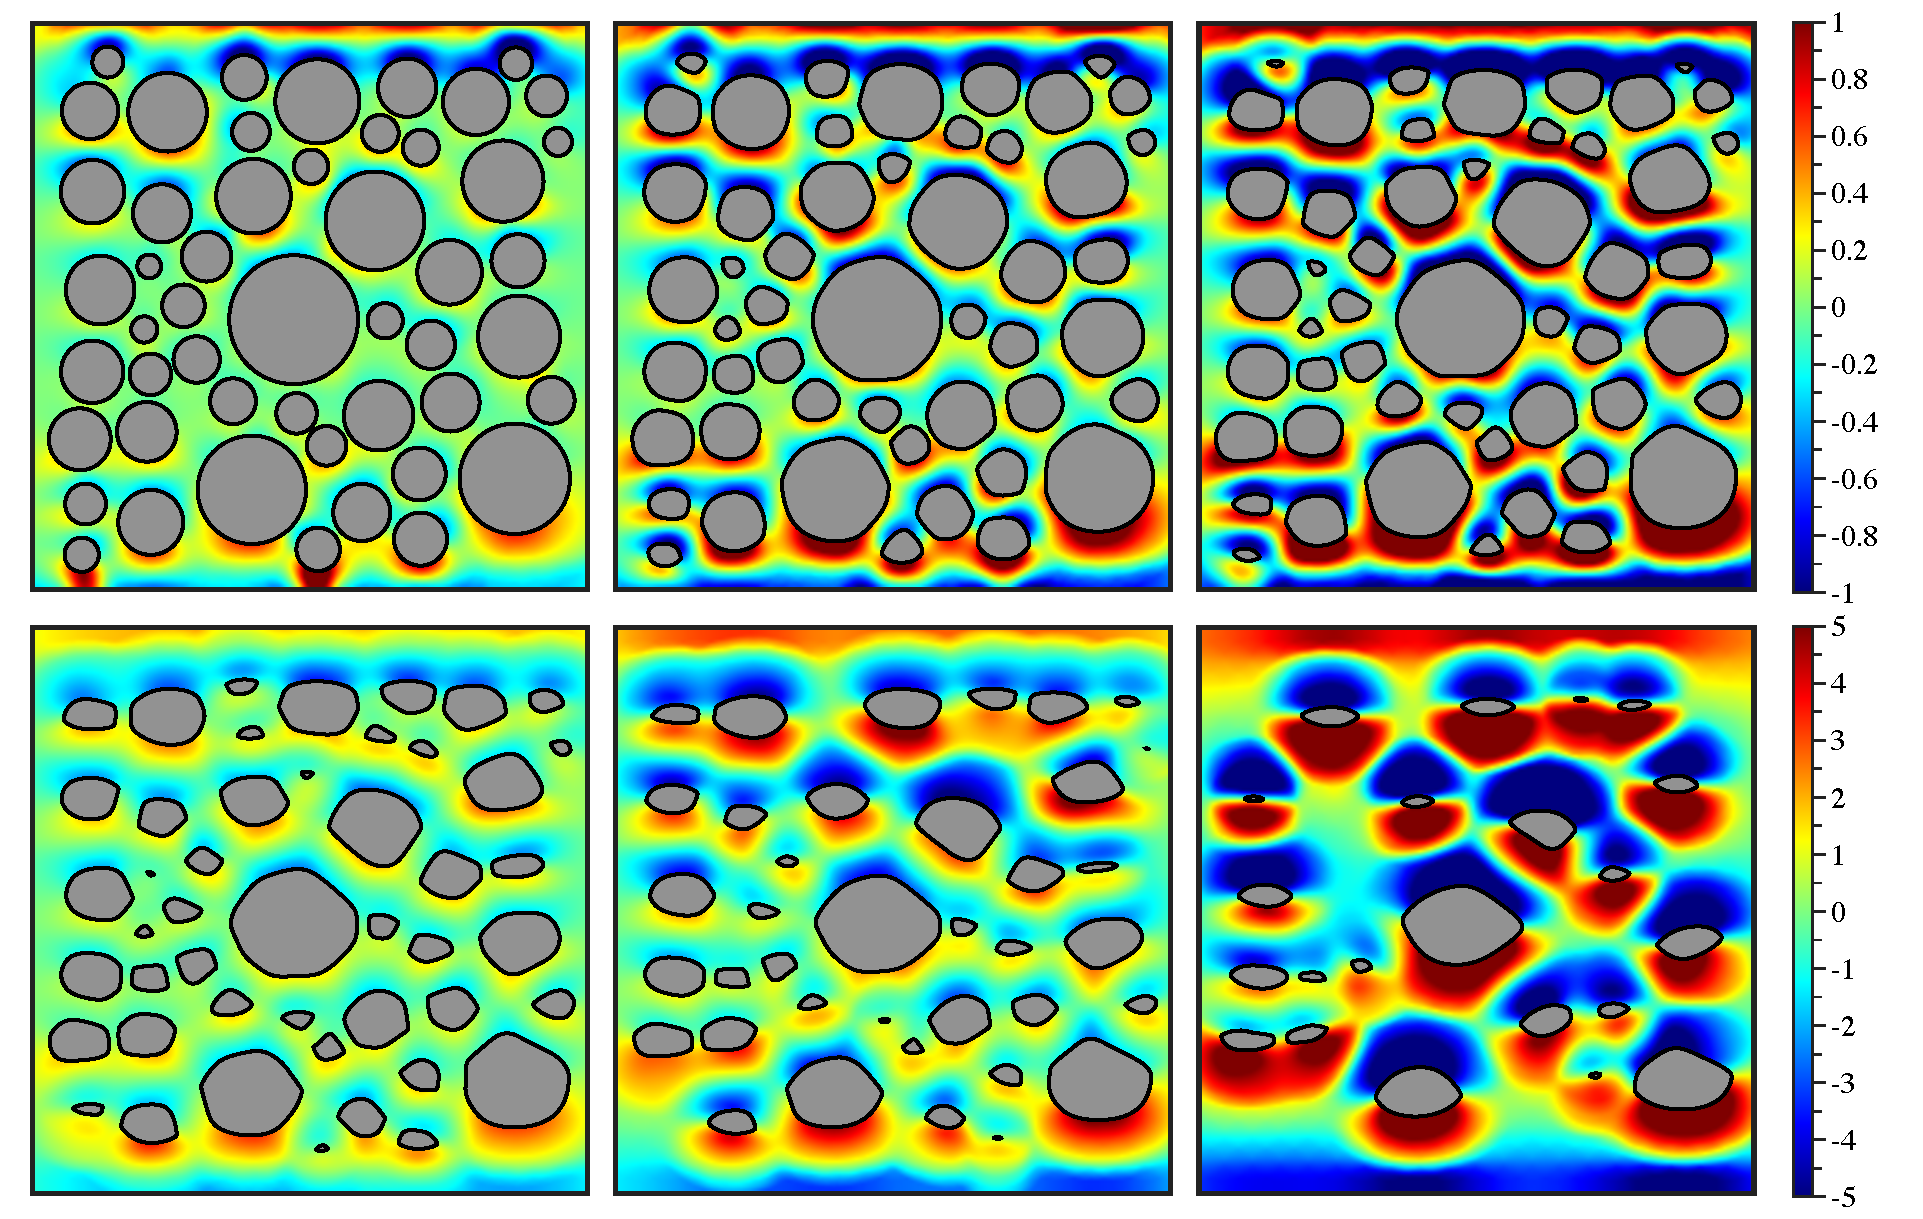
\includegraphics[width=0.58\textwidth]{figs/50bod.pdf}
\caption{\label{fig:50bod} \em Simulation of 50 bodies eroding in Stokes
flow under the action of fluid-mechanical erosion. The flow is
horizontal (left to right) and the 6 snapshots are evenly spaced in
time.  The local erosion rate on the bodies is proportional to the
magnitude of the vorticity which we compute in the fluid bulk (color
scale).  Erosion both diminishes the size of the bodies and considerably
alters their shapes.}
\end{wrapfigure}

Flow-induced erosion deteriorates and reshapes solid material over a
range of scales found in nature, including massive land formations
(mountains undergoing wind erosion) and watercourses (rivers and streams
undergoing hydraulic erosion).  Though less visible, erosion is working
at the very smallest scales, slowly deteriorating the individual
constituents of porous media (e.g.~soil, sand, or clay) or biological
structures like plaque and biofilms. Motivated by such examples, we are
interested in studying fluid-mechanical erosion in Stokes flow---the
most relevant regime for groundwater and bio-fluid applications.

In our recent publication~\cite{qua-moo2018}, we describe a suite of
numerical methods to simulate erosion in a viscous fluid
(Figure~\ref{fig:50bod}).  The highlights of our numerical methods are:
\begin{enumerate}[topsep=0pt,itemsep=-1ex,partopsep=1ex,parsep=1ex]
  \item {\bf Boundary Integral Equation Fluid Solver}: The
  fluid equations are solved with a boundary integral equation (BIE).
  The BIE formulation achives high-order accuracy in complex geometries
  with optimal computational complexity.

  \item {\bf Regularizations of the Interface}: Erosion results in
  numerically challenging corners of the bodies.  We use a
  regularization term and a smoothing operation to control the
  smoothness of the moving interface.

  \item {\bf Interface Tracking}: We describe the interface using
  {\thL} coordinates, where $\theta$ is a local tangent angle, and $L$
  is the total interface length.  In these coordinates, the
  stiff terms are linear which allows implicit methods to be used for time discretization.

  \item {\bf Validation}: We compare the numerical simulations against analytical predictions for the limiting shape of a single body and scaling laws for its vanishing rate.
\end{enumerate}

\section{Proposed Work}
Having developed and validated numerical methods for simulating viscous
erosion, there are two main directions that our research will follow.
First, {\bf additional numerical tools are required to simulate more
realistic scenarios such as denser packings, transport, and
three-dimensional erosion}.  Second, {\bf we will investigate physically
motivated questions regarding the reconfiguration of geometry and flow inside an eroding
porous medium}.

%%%%%%%%%%%%%%%%%%%%%%%%%%%%%%%%%%%%%%%%%%%%%%%%%%%%%%%%%%%%%%%%%%%%%%%%%%%%%
\subsection{Improved Numerical Methods}
\begin{wrapfigure}[22]{r}{0.4\textwidth}
\centering
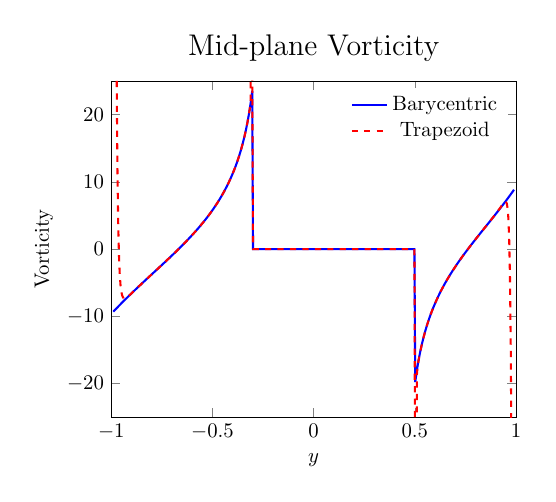
\begin{tikzpicture}[scale=0.75] 

\begin{axis}[ 
xmin=-1, 
xmax=1, 
%xtick = {0,3.1416,6.2832},
%xticklabels = {},
ymin=-25, 
ymax=25, 
%ytick = {-1.5708,0,1.5708,3.1416,4.7124,6.2832},
%yticklabels = {$-\frac{\pi}{2}$,$0$,$\frac{\pi}{2}$,$\pi$,$\frac{3\pi}{2}$,$2\pi$},
xlabel = {$y$},
ylabel = {Vorticity},
title = {\Large Mid-plane Vorticity},
legend style={draw=none}
] 

% vorticity in midplane
\addplot [color=blue,line width=1] coordinates{ 
(-9.9000e-01,-9.3147e+00)
(-9.8603e-01,-9.1881e+00)
(-9.8206e-01,-9.0621e+00)
(-9.7810e-01,-8.9368e+00)
(-9.7413e-01,-8.8121e+00)
(-9.7016e-01,-8.6881e+00)
(-9.6619e-01,-8.5647e+00)
(-9.6222e-01,-8.4419e+00)
(-9.5826e-01,-8.3197e+00)
(-9.5429e-01,-8.1981e+00)
(-9.5032e-01,-8.0770e+00)
(-9.4635e-01,-7.9564e+00)
(-9.4238e-01,-7.8364e+00)
(-9.3842e-01,-7.7169e+00)
(-9.3445e-01,-7.5979e+00)
(-9.3048e-01,-7.4793e+00)
(-9.2651e-01,-7.3612e+00)
(-9.2255e-01,-7.2436e+00)
(-9.1858e-01,-7.1264e+00)
(-9.1461e-01,-7.0096e+00)
(-9.1064e-01,-6.8932e+00)
(-9.0667e-01,-6.7772e+00)
(-9.0271e-01,-6.6616e+00)
(-8.9874e-01,-6.5464e+00)
(-8.9477e-01,-6.4315e+00)
(-8.9080e-01,-6.3169e+00)
(-8.8683e-01,-6.2027e+00)
(-8.8287e-01,-6.0888e+00)
(-8.7890e-01,-5.9752e+00)
(-8.7493e-01,-5.8618e+00)
(-8.7096e-01,-5.7488e+00)
(-8.6699e-01,-5.6360e+00)
(-8.6303e-01,-5.5234e+00)
(-8.5906e-01,-5.4111e+00)
(-8.5509e-01,-5.2990e+00)
(-8.5112e-01,-5.1870e+00)
(-8.4715e-01,-5.0753e+00)
(-8.4319e-01,-4.9638e+00)
(-8.3922e-01,-4.8524e+00)
(-8.3525e-01,-4.7412e+00)
(-8.3128e-01,-4.6302e+00)
(-8.2731e-01,-4.5192e+00)
(-8.2335e-01,-4.4084e+00)
(-8.1938e-01,-4.2977e+00)
(-8.1541e-01,-4.1870e+00)
(-8.1144e-01,-4.0765e+00)
(-8.0747e-01,-3.9660e+00)
(-8.0351e-01,-3.8556e+00)
(-7.9954e-01,-3.7452e+00)
(-7.9557e-01,-3.6348e+00)
(-7.9160e-01,-3.5245e+00)
(-7.8764e-01,-3.4141e+00)
(-7.8367e-01,-3.3037e+00)
(-7.7970e-01,-3.1933e+00)
(-7.7573e-01,-3.0829e+00)
(-7.7176e-01,-2.9724e+00)
(-7.6780e-01,-2.8619e+00)
(-7.6383e-01,-2.7512e+00)
(-7.5986e-01,-2.6405e+00)
(-7.5589e-01,-2.5297e+00)
(-7.5192e-01,-2.4187e+00)
(-7.4796e-01,-2.3076e+00)
(-7.4399e-01,-2.1963e+00)
(-7.4002e-01,-2.0849e+00)
(-7.3605e-01,-1.9733e+00)
(-7.3208e-01,-1.8615e+00)
(-7.2812e-01,-1.7495e+00)
(-7.2415e-01,-1.6373e+00)
(-7.2018e-01,-1.5248e+00)
(-7.1621e-01,-1.4120e+00)
(-7.1224e-01,-1.2990e+00)
(-7.0828e-01,-1.1857e+00)
(-7.0431e-01,-1.0721e+00)
(-7.0034e-01,-9.5814e-01)
(-6.9637e-01,-8.4385e-01)
(-6.9240e-01,-7.2919e-01)
(-6.8844e-01,-6.1416e-01)
(-6.8447e-01,-4.9872e-01)
(-6.8050e-01,-3.8287e-01)
(-6.7653e-01,-2.6658e-01)
(-6.7257e-01,-1.4983e-01)
(-6.6860e-01,-3.2599e-02)
(-6.6463e-01,8.5126e-02)
(-6.6066e-01,2.0337e-01)
(-6.5669e-01,3.2216e-01)
(-6.5273e-01,4.4151e-01)
(-6.4876e-01,5.6145e-01)
(-6.4479e-01,6.8200e-01)
(-6.4082e-01,8.0318e-01)
(-6.3685e-01,9.2502e-01)
(-6.3289e-01,1.0475e+00)
(-6.2892e-01,1.1708e+00)
(-6.2495e-01,1.2948e+00)
(-6.2098e-01,1.4195e+00)
(-6.1701e-01,1.5450e+00)
(-6.1305e-01,1.6714e+00)
(-6.0908e-01,1.7986e+00)
(-6.0511e-01,1.9267e+00)
(-6.0114e-01,2.0557e+00)
(-5.9717e-01,2.1857e+00)
(-5.9321e-01,2.3167e+00)
(-5.8924e-01,2.4486e+00)
(-5.8527e-01,2.5817e+00)
(-5.8130e-01,2.7158e+00)
(-5.7733e-01,2.8511e+00)
(-5.7337e-01,2.9876e+00)
(-5.6940e-01,3.1252e+00)
(-5.6543e-01,3.2642e+00)
(-5.6146e-01,3.4045e+00)
(-5.5749e-01,3.5461e+00)
(-5.5353e-01,3.6891e+00)
(-5.4956e-01,3.8336e+00)
(-5.4559e-01,3.9796e+00)
(-5.4162e-01,4.1272e+00)
(-5.3766e-01,4.2764e+00)
(-5.3369e-01,4.4274e+00)
(-5.2972e-01,4.5800e+00)
(-5.2575e-01,4.7346e+00)
(-5.2178e-01,4.8910e+00)
(-5.1782e-01,5.0493e+00)
(-5.1385e-01,5.2098e+00)
(-5.0988e-01,5.3723e+00)
(-5.0591e-01,5.5371e+00)
(-5.0194e-01,5.7042e+00)
(-4.9798e-01,5.8737e+00)
(-4.9401e-01,6.0456e+00)
(-4.9004e-01,6.2202e+00)
(-4.8607e-01,6.3975e+00)
(-4.8210e-01,6.5776e+00)
(-4.7814e-01,6.7607e+00)
(-4.7417e-01,6.9469e+00)
(-4.7020e-01,7.1362e+00)
(-4.6623e-01,7.3290e+00)
(-4.6226e-01,7.5252e+00)
(-4.5830e-01,7.7252e+00)
(-4.5433e-01,7.9290e+00)
(-4.5036e-01,8.1368e+00)
(-4.4639e-01,8.3489e+00)
(-4.4242e-01,8.5654e+00)
(-4.3846e-01,8.7866e+00)
(-4.3449e-01,9.0127e+00)
(-4.3052e-01,9.2440e+00)
(-4.2655e-01,9.4807e+00)
(-4.2259e-01,9.7232e+00)
(-4.1862e-01,9.9718e+00)
(-4.1465e-01,1.0227e+01)
(-4.1068e-01,1.0489e+01)
(-4.0671e-01,1.0758e+01)
(-4.0275e-01,1.1034e+01)
(-3.9878e-01,1.1319e+01)
(-3.9481e-01,1.1612e+01)
(-3.9084e-01,1.1915e+01)
(-3.8687e-01,1.2227e+01)
(-3.8291e-01,1.2550e+01)
(-3.7894e-01,1.2885e+01)
(-3.7497e-01,1.3231e+01)
(-3.7100e-01,1.3590e+01)
(-3.6703e-01,1.3964e+01)
(-3.6307e-01,1.4352e+01)
(-3.5910e-01,1.4758e+01)
(-3.5513e-01,1.5181e+01)
(-3.5116e-01,1.5623e+01)
(-3.4719e-01,1.6087e+01)
(-3.4323e-01,1.6575e+01)
(-3.3926e-01,1.7088e+01)
(-3.3529e-01,1.7630e+01)
(-3.3132e-01,1.8203e+01)
(-3.2735e-01,1.8813e+01)
(-3.2339e-01,1.9461e+01)
(-3.1942e-01,2.0155e+01)
(-3.1545e-01,2.0900e+01)
(-3.1148e-01,2.1704e+01)
(-3.0752e-01,2.2575e+01)
(-3.0355e-01,2.3525e+01)
(-2.9958e-01,0.0000e+00)
(-2.9561e-01,0.0000e+00)
(-2.9164e-01,0.0000e+00)
(-2.8768e-01,0.0000e+00)
(-2.8371e-01,0.0000e+00)
(-2.7974e-01,0.0000e+00)
(-2.7577e-01,0.0000e+00)
(-2.7180e-01,0.0000e+00)
(-2.6784e-01,0.0000e+00)
(-2.6387e-01,0.0000e+00)
(-2.5990e-01,0.0000e+00)
(-2.5593e-01,0.0000e+00)
(-2.5196e-01,0.0000e+00)
(-2.4800e-01,0.0000e+00)
(-2.4403e-01,0.0000e+00)
(-2.4006e-01,0.0000e+00)
(-2.3609e-01,0.0000e+00)
(-2.3212e-01,0.0000e+00)
(-2.2816e-01,0.0000e+00)
(-2.2419e-01,0.0000e+00)
(-2.2022e-01,0.0000e+00)
(-2.1625e-01,0.0000e+00)
(-2.1228e-01,0.0000e+00)
(-2.0832e-01,0.0000e+00)
(-2.0435e-01,0.0000e+00)
(-2.0038e-01,0.0000e+00)
(-1.9641e-01,0.0000e+00)
(-1.9244e-01,0.0000e+00)
(-1.8848e-01,0.0000e+00)
(-1.8451e-01,0.0000e+00)
(-1.8054e-01,0.0000e+00)
(-1.7657e-01,0.0000e+00)
(-1.7261e-01,0.0000e+00)
(-1.6864e-01,0.0000e+00)
(-1.6467e-01,0.0000e+00)
(-1.6070e-01,0.0000e+00)
(-1.5673e-01,0.0000e+00)
(-1.5277e-01,0.0000e+00)
(-1.4880e-01,0.0000e+00)
(-1.4483e-01,0.0000e+00)
(-1.4086e-01,0.0000e+00)
(-1.3689e-01,0.0000e+00)
(-1.3293e-01,0.0000e+00)
(-1.2896e-01,0.0000e+00)
(-1.2499e-01,0.0000e+00)
(-1.2102e-01,0.0000e+00)
(-1.1705e-01,0.0000e+00)
(-1.1309e-01,0.0000e+00)
(-1.0912e-01,0.0000e+00)
(-1.0515e-01,0.0000e+00)
(-1.0118e-01,0.0000e+00)
(-9.7214e-02,0.0000e+00)
(-9.3246e-02,0.0000e+00)
(-8.9279e-02,0.0000e+00)
(-8.5311e-02,0.0000e+00)
(-8.1343e-02,0.0000e+00)
(-7.7375e-02,0.0000e+00)
(-7.3407e-02,0.0000e+00)
(-6.9439e-02,0.0000e+00)
(-6.5471e-02,0.0000e+00)
(-6.1503e-02,0.0000e+00)
(-5.7535e-02,0.0000e+00)
(-5.3567e-02,0.0000e+00)
(-4.9599e-02,0.0000e+00)
(-4.5631e-02,0.0000e+00)
(-4.1663e-02,0.0000e+00)
(-3.7695e-02,0.0000e+00)
(-3.3727e-02,0.0000e+00)
(-2.9760e-02,0.0000e+00)
(-2.5792e-02,0.0000e+00)
(-2.1824e-02,0.0000e+00)
(-1.7856e-02,0.0000e+00)
(-1.3888e-02,0.0000e+00)
(-9.9198e-03,0.0000e+00)
(-5.9519e-03,0.0000e+00)
(-1.9840e-03,0.0000e+00)
(1.9840e-03,0.0000e+00)
(5.9519e-03,0.0000e+00)
(9.9198e-03,0.0000e+00)
(1.3888e-02,0.0000e+00)
(1.7856e-02,0.0000e+00)
(2.1824e-02,0.0000e+00)
(2.5792e-02,0.0000e+00)
(2.9760e-02,0.0000e+00)
(3.3727e-02,0.0000e+00)
(3.7695e-02,0.0000e+00)
(4.1663e-02,0.0000e+00)
(4.5631e-02,0.0000e+00)
(4.9599e-02,0.0000e+00)
(5.3567e-02,0.0000e+00)
(5.7535e-02,0.0000e+00)
(6.1503e-02,0.0000e+00)
(6.5471e-02,0.0000e+00)
(6.9439e-02,0.0000e+00)
(7.3407e-02,0.0000e+00)
(7.7375e-02,0.0000e+00)
(8.1343e-02,0.0000e+00)
(8.5311e-02,0.0000e+00)
(8.9279e-02,0.0000e+00)
(9.3246e-02,0.0000e+00)
(9.7214e-02,0.0000e+00)
(1.0118e-01,0.0000e+00)
(1.0515e-01,0.0000e+00)
(1.0912e-01,0.0000e+00)
(1.1309e-01,0.0000e+00)
(1.1705e-01,0.0000e+00)
(1.2102e-01,0.0000e+00)
(1.2499e-01,0.0000e+00)
(1.2896e-01,0.0000e+00)
(1.3293e-01,0.0000e+00)
(1.3689e-01,0.0000e+00)
(1.4086e-01,0.0000e+00)
(1.4483e-01,0.0000e+00)
(1.4880e-01,0.0000e+00)
(1.5277e-01,0.0000e+00)
(1.5673e-01,0.0000e+00)
(1.6070e-01,0.0000e+00)
(1.6467e-01,0.0000e+00)
(1.6864e-01,0.0000e+00)
(1.7261e-01,0.0000e+00)
(1.7657e-01,0.0000e+00)
(1.8054e-01,0.0000e+00)
(1.8451e-01,0.0000e+00)
(1.8848e-01,0.0000e+00)
(1.9244e-01,0.0000e+00)
(1.9641e-01,0.0000e+00)
(2.0038e-01,0.0000e+00)
(2.0435e-01,0.0000e+00)
(2.0832e-01,0.0000e+00)
(2.1228e-01,0.0000e+00)
(2.1625e-01,0.0000e+00)
(2.2022e-01,0.0000e+00)
(2.2419e-01,0.0000e+00)
(2.2816e-01,0.0000e+00)
(2.3212e-01,0.0000e+00)
(2.3609e-01,0.0000e+00)
(2.4006e-01,0.0000e+00)
(2.4403e-01,0.0000e+00)
(2.4800e-01,0.0000e+00)
(2.5196e-01,0.0000e+00)
(2.5593e-01,0.0000e+00)
(2.5990e-01,0.0000e+00)
(2.6387e-01,0.0000e+00)
(2.6784e-01,0.0000e+00)
(2.7180e-01,0.0000e+00)
(2.7577e-01,0.0000e+00)
(2.7974e-01,0.0000e+00)
(2.8371e-01,0.0000e+00)
(2.8768e-01,0.0000e+00)
(2.9164e-01,0.0000e+00)
(2.9561e-01,0.0000e+00)
(2.9958e-01,0.0000e+00)
(3.0355e-01,0.0000e+00)
(3.0752e-01,0.0000e+00)
(3.1148e-01,0.0000e+00)
(3.1545e-01,0.0000e+00)
(3.1942e-01,0.0000e+00)
(3.2339e-01,0.0000e+00)
(3.2735e-01,0.0000e+00)
(3.3132e-01,0.0000e+00)
(3.3529e-01,0.0000e+00)
(3.3926e-01,0.0000e+00)
(3.4323e-01,0.0000e+00)
(3.4719e-01,0.0000e+00)
(3.5116e-01,0.0000e+00)
(3.5513e-01,0.0000e+00)
(3.5910e-01,0.0000e+00)
(3.6307e-01,0.0000e+00)
(3.6703e-01,0.0000e+00)
(3.7100e-01,0.0000e+00)
(3.7497e-01,0.0000e+00)
(3.7894e-01,0.0000e+00)
(3.8291e-01,0.0000e+00)
(3.8687e-01,0.0000e+00)
(3.9084e-01,0.0000e+00)
(3.9481e-01,0.0000e+00)
(3.9878e-01,0.0000e+00)
(4.0275e-01,0.0000e+00)
(4.0671e-01,0.0000e+00)
(4.1068e-01,0.0000e+00)
(4.1465e-01,0.0000e+00)
(4.1862e-01,0.0000e+00)
(4.2259e-01,0.0000e+00)
(4.2655e-01,0.0000e+00)
(4.3052e-01,0.0000e+00)
(4.3449e-01,0.0000e+00)
(4.3846e-01,0.0000e+00)
(4.4242e-01,0.0000e+00)
(4.4639e-01,0.0000e+00)
(4.5036e-01,0.0000e+00)
(4.5433e-01,0.0000e+00)
(4.5830e-01,0.0000e+00)
(4.6226e-01,0.0000e+00)
(4.6623e-01,0.0000e+00)
(4.7020e-01,0.0000e+00)
(4.7417e-01,0.0000e+00)
(4.7814e-01,0.0000e+00)
(4.8210e-01,0.0000e+00)
(4.8607e-01,0.0000e+00)
(4.9004e-01,0.0000e+00)
(4.9401e-01,0.0000e+00)
(4.9798e-01,0.0000e+00)
(5.0194e-01,-1.9785e+01)
(5.0591e-01,-1.8904e+01)
(5.0988e-01,-1.8095e+01)
(5.1385e-01,-1.7347e+01)
(5.1782e-01,-1.6654e+01)
(5.2178e-01,-1.6007e+01)
(5.2575e-01,-1.5401e+01)
(5.2972e-01,-1.4831e+01)
(5.3369e-01,-1.4294e+01)
(5.3766e-01,-1.3785e+01)
(5.4162e-01,-1.3302e+01)
(5.4559e-01,-1.2843e+01)
(5.4956e-01,-1.2404e+01)
(5.5353e-01,-1.1985e+01)
(5.5749e-01,-1.1583e+01)
(5.6146e-01,-1.1198e+01)
(5.6543e-01,-1.0827e+01)
(5.6940e-01,-1.0470e+01)
(5.7337e-01,-1.0126e+01)
(5.7733e-01,-9.7929e+00)
(5.8130e-01,-9.4709e+00)
(5.8527e-01,-9.1589e+00)
(5.8924e-01,-8.8563e+00)
(5.9321e-01,-8.5625e+00)
(5.9717e-01,-8.2768e+00)
(6.0114e-01,-7.9987e+00)
(6.0511e-01,-7.7279e+00)
(6.0908e-01,-7.4638e+00)
(6.1305e-01,-7.2060e+00)
(6.1701e-01,-6.9542e+00)
(6.2098e-01,-6.7080e+00)
(6.2495e-01,-6.4671e+00)
(6.2892e-01,-6.2312e+00)
(6.3289e-01,-6.0001e+00)
(6.3685e-01,-5.7735e+00)
(6.4082e-01,-5.5511e+00)
(6.4479e-01,-5.3328e+00)
(6.4876e-01,-5.1183e+00)
(6.5273e-01,-4.9074e+00)
(6.5669e-01,-4.7000e+00)
(6.6066e-01,-4.4958e+00)
(6.6463e-01,-4.2948e+00)
(6.6860e-01,-4.0967e+00)
(6.7257e-01,-3.9014e+00)
(6.7653e-01,-3.7088e+00)
(6.8050e-01,-3.5188e+00)
(6.8447e-01,-3.3312e+00)
(6.8844e-01,-3.1460e+00)
(6.9240e-01,-2.9629e+00)
(6.9637e-01,-2.7820e+00)
(7.0034e-01,-2.6030e+00)
(7.0431e-01,-2.4260e+00)
(7.0828e-01,-2.2508e+00)
(7.1224e-01,-2.0774e+00)
(7.1621e-01,-1.9056e+00)
(7.2018e-01,-1.7353e+00)
(7.2415e-01,-1.5666e+00)
(7.2812e-01,-1.3993e+00)
(7.3208e-01,-1.2334e+00)
(7.3605e-01,-1.0687e+00)
(7.4002e-01,-9.0533e-01)
(7.4399e-01,-7.4309e-01)
(7.4796e-01,-5.8195e-01)
(7.5192e-01,-4.2186e-01)
(7.5589e-01,-2.6277e-01)
(7.5986e-01,-1.0462e-01)
(7.6383e-01,5.2637e-02)
(7.6780e-01,2.0906e-01)
(7.7176e-01,3.6469e-01)
(7.7573e-01,5.1958e-01)
(7.7970e-01,6.7377e-01)
(7.8367e-01,8.2732e-01)
(7.8764e-01,9.8025e-01)
(7.9160e-01,1.1326e+00)
(7.9557e-01,1.2845e+00)
(7.9954e-01,1.4358e+00)
(8.0351e-01,1.5868e+00)
(8.0747e-01,1.7373e+00)
(8.1144e-01,1.8874e+00)
(8.1541e-01,2.0373e+00)
(8.1938e-01,2.1868e+00)
(8.2335e-01,2.3361e+00)
(8.2731e-01,2.4852e+00)
(8.3128e-01,2.6340e+00)
(8.3525e-01,2.7828e+00)
(8.3922e-01,2.9314e+00)
(8.4319e-01,3.0799e+00)
(8.4715e-01,3.2284e+00)
(8.5112e-01,3.3769e+00)
(8.5509e-01,3.5254e+00)
(8.5906e-01,3.6739e+00)
(8.6303e-01,3.8226e+00)
(8.6699e-01,3.9713e+00)
(8.7096e-01,4.1202e+00)
(8.7493e-01,4.2693e+00)
(8.7890e-01,4.4186e+00)
(8.8287e-01,4.5681e+00)
(8.8683e-01,4.7180e+00)
(8.9080e-01,4.8681e+00)
(8.9477e-01,5.0185e+00)
(8.9874e-01,5.1694e+00)
(9.0271e-01,5.3206e+00)
(9.0667e-01,5.4723e+00)
(9.1064e-01,5.6244e+00)
(9.1461e-01,5.7771e+00)
(9.1858e-01,5.9302e+00)
(9.2255e-01,6.0840e+00)
(9.2651e-01,6.2383e+00)
(9.3048e-01,6.3933e+00)
(9.3445e-01,6.5490e+00)
(9.3842e-01,6.7053e+00)
(9.4238e-01,6.8624e+00)
(9.4635e-01,7.0202e+00)
(9.5032e-01,7.1789e+00)
(9.5429e-01,7.3384e+00)
(9.5826e-01,7.4988e+00)
(9.6222e-01,7.6601e+00)
(9.6619e-01,7.8224e+00)
(9.7016e-01,7.9856e+00)
(9.7413e-01,8.1499e+00)
(9.7810e-01,8.3152e+00)
(9.8206e-01,8.4817e+00)
(9.8603e-01,8.6493e+00)
(9.9000e-01,8.8181e+00)
}; 
\addlegendentry{Barycentric}

\addplot [color=red,dashed,line width=1] coordinates{ 
%(-9.9000e-01,2.4932e+02)
%(-9.8603e-01,1.6180e+02)
%(-9.8206e-01,9.7328e+01)
%(-9.7810e-01,5.4851e+01)
(-9.7413e-01,2.8715e+01)
(-9.7016e-01,1.3259e+01)
(-9.6619e-01,4.3108e+00)
(-9.6222e-01,-8.2074e-01)
(-9.5826e-01,-3.7532e+00)
(-9.5429e-01,-5.4250e+00)
(-9.5032e-01,-6.3710e+00)
(-9.4635e-01,-6.8951e+00)
(-9.4238e-01,-7.1704e+00)
(-9.3842e-01,-7.2966e+00)
(-9.3445e-01,-7.3322e+00)
(-9.3048e-01,-7.3117e+00)
(-9.2651e-01,-7.2562e+00)
(-9.2255e-01,-7.1785e+00)
(-9.1858e-01,-7.0868e+00)
(-9.1461e-01,-6.9862e+00)
(-9.1064e-01,-6.8800e+00)
(-9.0667e-01,-6.7703e+00)
(-9.0271e-01,-6.6585e+00)
(-8.9874e-01,-6.5455e+00)
(-8.9477e-01,-6.4318e+00)
(-8.9080e-01,-6.3179e+00)
(-8.8683e-01,-6.2039e+00)
(-8.8287e-01,-6.0900e+00)
(-8.7890e-01,-5.9764e+00)
(-8.7493e-01,-5.8629e+00)
(-8.7096e-01,-5.7497e+00)
(-8.6699e-01,-5.6367e+00)
(-8.6303e-01,-5.5240e+00)
(-8.5906e-01,-5.4116e+00)
(-8.5509e-01,-5.2994e+00)
(-8.5112e-01,-5.1874e+00)
(-8.4715e-01,-5.0756e+00)
(-8.4319e-01,-4.9640e+00)
(-8.3922e-01,-4.8526e+00)
(-8.3525e-01,-4.7413e+00)
(-8.3128e-01,-4.6302e+00)
(-8.2731e-01,-4.5193e+00)
(-8.2335e-01,-4.4084e+00)
(-8.1938e-01,-4.2977e+00)
(-8.1541e-01,-4.1871e+00)
(-8.1144e-01,-4.0765e+00)
(-8.0747e-01,-3.9660e+00)
(-8.0351e-01,-3.8556e+00)
(-7.9954e-01,-3.7452e+00)
(-7.9557e-01,-3.6348e+00)
(-7.9160e-01,-3.5245e+00)
(-7.8764e-01,-3.4141e+00)
(-7.8367e-01,-3.3037e+00)
(-7.7970e-01,-3.1934e+00)
(-7.7573e-01,-3.0829e+00)
(-7.7176e-01,-2.9724e+00)
(-7.6780e-01,-2.8619e+00)
(-7.6383e-01,-2.7512e+00)
(-7.5986e-01,-2.6405e+00)
(-7.5589e-01,-2.5297e+00)
(-7.5192e-01,-2.4187e+00)
(-7.4796e-01,-2.3076e+00)
(-7.4399e-01,-2.1963e+00)
(-7.4002e-01,-2.0849e+00)
(-7.3605e-01,-1.9733e+00)
(-7.3208e-01,-1.8615e+00)
(-7.2812e-01,-1.7495e+00)
(-7.2415e-01,-1.6373e+00)
(-7.2018e-01,-1.5248e+00)
(-7.1621e-01,-1.4120e+00)
(-7.1224e-01,-1.2990e+00)
(-7.0828e-01,-1.1857e+00)
(-7.0431e-01,-1.0721e+00)
(-7.0034e-01,-9.5814e-01)
(-6.9637e-01,-8.4385e-01)
(-6.9240e-01,-7.2919e-01)
(-6.8844e-01,-6.1416e-01)
(-6.8447e-01,-4.9872e-01)
(-6.8050e-01,-3.8287e-01)
(-6.7653e-01,-2.6658e-01)
(-6.7257e-01,-1.4983e-01)
(-6.6860e-01,-3.2599e-02)
(-6.6463e-01,8.5126e-02)
(-6.6066e-01,2.0337e-01)
(-6.5669e-01,3.2216e-01)
(-6.5273e-01,4.4151e-01)
(-6.4876e-01,5.6145e-01)
(-6.4479e-01,6.8200e-01)
(-6.4082e-01,8.0318e-01)
(-6.3685e-01,9.2502e-01)
(-6.3289e-01,1.0475e+00)
(-6.2892e-01,1.1708e+00)
(-6.2495e-01,1.2948e+00)
(-6.2098e-01,1.4195e+00)
(-6.1701e-01,1.5450e+00)
(-6.1305e-01,1.6714e+00)
(-6.0908e-01,1.7986e+00)
(-6.0511e-01,1.9267e+00)
(-6.0114e-01,2.0557e+00)
(-5.9717e-01,2.1857e+00)
(-5.9321e-01,2.3167e+00)
(-5.8924e-01,2.4486e+00)
(-5.8527e-01,2.5817e+00)
(-5.8130e-01,2.7158e+00)
(-5.7733e-01,2.8511e+00)
(-5.7337e-01,2.9876e+00)
(-5.6940e-01,3.1252e+00)
(-5.6543e-01,3.2642e+00)
(-5.6146e-01,3.4045e+00)
(-5.5749e-01,3.5461e+00)
(-5.5353e-01,3.6891e+00)
(-5.4956e-01,3.8336e+00)
(-5.4559e-01,3.9796e+00)
(-5.4162e-01,4.1272e+00)
(-5.3766e-01,4.2764e+00)
(-5.3369e-01,4.4274e+00)
(-5.2972e-01,4.5800e+00)
(-5.2575e-01,4.7346e+00)
(-5.2178e-01,4.8910e+00)
(-5.1782e-01,5.0493e+00)
(-5.1385e-01,5.2098e+00)
(-5.0988e-01,5.3723e+00)
(-5.0591e-01,5.5371e+00)
(-5.0194e-01,5.7042e+00)
(-4.9798e-01,5.8737e+00)
(-4.9401e-01,6.0456e+00)
(-4.9004e-01,6.2202e+00)
(-4.8607e-01,6.3975e+00)
(-4.8210e-01,6.5776e+00)
(-4.7814e-01,6.7607e+00)
(-4.7417e-01,6.9469e+00)
(-4.7020e-01,7.1362e+00)
(-4.6623e-01,7.3290e+00)
(-4.6226e-01,7.5252e+00)
(-4.5830e-01,7.7252e+00)
(-4.5433e-01,7.9290e+00)
(-4.5036e-01,8.1368e+00)
(-4.4639e-01,8.3489e+00)
(-4.4242e-01,8.5654e+00)
(-4.3846e-01,8.7866e+00)
(-4.3449e-01,9.0127e+00)
(-4.3052e-01,9.2440e+00)
(-4.2655e-01,9.4807e+00)
(-4.2259e-01,9.7232e+00)
(-4.1862e-01,9.9718e+00)
(-4.1465e-01,1.0227e+01)
(-4.1068e-01,1.0489e+01)
(-4.0671e-01,1.0758e+01)
(-4.0275e-01,1.1034e+01)
(-3.9878e-01,1.1319e+01)
(-3.9481e-01,1.1612e+01)
(-3.9084e-01,1.1915e+01)
(-3.8687e-01,1.2227e+01)
(-3.8291e-01,1.2550e+01)
(-3.7894e-01,1.2885e+01)
(-3.7497e-01,1.3231e+01)
(-3.7100e-01,1.3590e+01)
(-3.6703e-01,1.3964e+01)
(-3.6307e-01,1.4352e+01)
(-3.5910e-01,1.4758e+01)
(-3.5513e-01,1.5181e+01)
(-3.5116e-01,1.5623e+01)
(-3.4719e-01,1.6087e+01)
(-3.4323e-01,1.6575e+01)
(-3.3926e-01,1.7088e+01)
(-3.3529e-01,1.7630e+01)
(-3.3132e-01,1.8203e+01)
(-3.2735e-01,1.8813e+01)
(-3.2339e-01,1.9461e+01)
(-3.1942e-01,2.0155e+01)
(-3.1545e-01,2.0904e+01)
(-3.1148e-01,2.2008e+01)
(-3.0752e-01,5.3646e+01)
%(-3.0355e-01,3.6442e+03)
(-2.9958e-01,0.0000e+00)
(-2.9561e-01,0.0000e+00)
(-2.9164e-01,0.0000e+00)
(-2.8768e-01,0.0000e+00)
(-2.8371e-01,0.0000e+00)
(-2.7974e-01,0.0000e+00)
(-2.7577e-01,0.0000e+00)
(-2.7180e-01,0.0000e+00)
(-2.6784e-01,0.0000e+00)
(-2.6387e-01,0.0000e+00)
(-2.5990e-01,0.0000e+00)
(-2.5593e-01,0.0000e+00)
(-2.5196e-01,0.0000e+00)
(-2.4800e-01,0.0000e+00)
(-2.4403e-01,0.0000e+00)
(-2.4006e-01,0.0000e+00)
(-2.3609e-01,0.0000e+00)
(-2.3212e-01,0.0000e+00)
(-2.2816e-01,0.0000e+00)
(-2.2419e-01,0.0000e+00)
(-2.2022e-01,0.0000e+00)
(-2.1625e-01,0.0000e+00)
(-2.1228e-01,0.0000e+00)
(-2.0832e-01,0.0000e+00)
(-2.0435e-01,0.0000e+00)
(-2.0038e-01,0.0000e+00)
(-1.9641e-01,0.0000e+00)
(-1.9244e-01,0.0000e+00)
(-1.8848e-01,0.0000e+00)
(-1.8451e-01,0.0000e+00)
(-1.8054e-01,0.0000e+00)
(-1.7657e-01,0.0000e+00)
(-1.7261e-01,0.0000e+00)
(-1.6864e-01,0.0000e+00)
(-1.6467e-01,0.0000e+00)
(-1.6070e-01,0.0000e+00)
(-1.5673e-01,0.0000e+00)
(-1.5277e-01,0.0000e+00)
(-1.4880e-01,0.0000e+00)
(-1.4483e-01,0.0000e+00)
(-1.4086e-01,0.0000e+00)
(-1.3689e-01,0.0000e+00)
(-1.3293e-01,0.0000e+00)
(-1.2896e-01,0.0000e+00)
(-1.2499e-01,0.0000e+00)
(-1.2102e-01,0.0000e+00)
(-1.1705e-01,0.0000e+00)
(-1.1309e-01,0.0000e+00)
(-1.0912e-01,0.0000e+00)
(-1.0515e-01,0.0000e+00)
(-1.0118e-01,0.0000e+00)
(-9.7214e-02,0.0000e+00)
(-9.3246e-02,0.0000e+00)
(-8.9279e-02,0.0000e+00)
(-8.5311e-02,0.0000e+00)
(-8.1343e-02,0.0000e+00)
(-7.7375e-02,0.0000e+00)
(-7.3407e-02,0.0000e+00)
(-6.9439e-02,0.0000e+00)
(-6.5471e-02,0.0000e+00)
(-6.1503e-02,0.0000e+00)
(-5.7535e-02,0.0000e+00)
(-5.3567e-02,0.0000e+00)
(-4.9599e-02,0.0000e+00)
(-4.5631e-02,0.0000e+00)
(-4.1663e-02,0.0000e+00)
(-3.7695e-02,0.0000e+00)
(-3.3727e-02,0.0000e+00)
(-2.9760e-02,0.0000e+00)
(-2.5792e-02,0.0000e+00)
(-2.1824e-02,0.0000e+00)
(-1.7856e-02,0.0000e+00)
(-1.3888e-02,0.0000e+00)
(-9.9198e-03,0.0000e+00)
(-5.9519e-03,0.0000e+00)
(-1.9840e-03,0.0000e+00)
(1.9840e-03,0.0000e+00)
(5.9519e-03,0.0000e+00)
(9.9198e-03,0.0000e+00)
(1.3888e-02,0.0000e+00)
(1.7856e-02,0.0000e+00)
(2.1824e-02,0.0000e+00)
(2.5792e-02,0.0000e+00)
(2.9760e-02,0.0000e+00)
(3.3727e-02,0.0000e+00)
(3.7695e-02,0.0000e+00)
(4.1663e-02,0.0000e+00)
(4.5631e-02,0.0000e+00)
(4.9599e-02,0.0000e+00)
(5.3567e-02,0.0000e+00)
(5.7535e-02,0.0000e+00)
(6.1503e-02,0.0000e+00)
(6.5471e-02,0.0000e+00)
(6.9439e-02,0.0000e+00)
(7.3407e-02,0.0000e+00)
(7.7375e-02,0.0000e+00)
(8.1343e-02,0.0000e+00)
(8.5311e-02,0.0000e+00)
(8.9279e-02,0.0000e+00)
(9.3246e-02,0.0000e+00)
(9.7214e-02,0.0000e+00)
(1.0118e-01,0.0000e+00)
(1.0515e-01,0.0000e+00)
(1.0912e-01,0.0000e+00)
(1.1309e-01,0.0000e+00)
(1.1705e-01,0.0000e+00)
(1.2102e-01,0.0000e+00)
(1.2499e-01,0.0000e+00)
(1.2896e-01,0.0000e+00)
(1.3293e-01,0.0000e+00)
(1.3689e-01,0.0000e+00)
(1.4086e-01,0.0000e+00)
(1.4483e-01,0.0000e+00)
(1.4880e-01,0.0000e+00)
(1.5277e-01,0.0000e+00)
(1.5673e-01,0.0000e+00)
(1.6070e-01,0.0000e+00)
(1.6467e-01,0.0000e+00)
(1.6864e-01,0.0000e+00)
(1.7261e-01,0.0000e+00)
(1.7657e-01,0.0000e+00)
(1.8054e-01,0.0000e+00)
(1.8451e-01,0.0000e+00)
(1.8848e-01,0.0000e+00)
(1.9244e-01,0.0000e+00)
(1.9641e-01,0.0000e+00)
(2.0038e-01,0.0000e+00)
(2.0435e-01,0.0000e+00)
(2.0832e-01,0.0000e+00)
(2.1228e-01,0.0000e+00)
(2.1625e-01,0.0000e+00)
(2.2022e-01,0.0000e+00)
(2.2419e-01,0.0000e+00)
(2.2816e-01,0.0000e+00)
(2.3212e-01,0.0000e+00)
(2.3609e-01,0.0000e+00)
(2.4006e-01,0.0000e+00)
(2.4403e-01,0.0000e+00)
(2.4800e-01,0.0000e+00)
(2.5196e-01,0.0000e+00)
(2.5593e-01,0.0000e+00)
(2.5990e-01,0.0000e+00)
(2.6387e-01,0.0000e+00)
(2.6784e-01,0.0000e+00)
(2.7180e-01,0.0000e+00)
(2.7577e-01,0.0000e+00)
(2.7974e-01,0.0000e+00)
(2.8371e-01,0.0000e+00)
(2.8768e-01,0.0000e+00)
(2.9164e-01,0.0000e+00)
(2.9561e-01,0.0000e+00)
(2.9958e-01,0.0000e+00)
(3.0355e-01,0.0000e+00)
(3.0752e-01,0.0000e+00)
(3.1148e-01,0.0000e+00)
(3.1545e-01,0.0000e+00)
(3.1942e-01,0.0000e+00)
(3.2339e-01,0.0000e+00)
(3.2735e-01,0.0000e+00)
(3.3132e-01,0.0000e+00)
(3.3529e-01,0.0000e+00)
(3.3926e-01,0.0000e+00)
(3.4323e-01,0.0000e+00)
(3.4719e-01,0.0000e+00)
(3.5116e-01,0.0000e+00)
(3.5513e-01,0.0000e+00)
(3.5910e-01,0.0000e+00)
(3.6307e-01,0.0000e+00)
(3.6703e-01,0.0000e+00)
(3.7100e-01,0.0000e+00)
(3.7497e-01,0.0000e+00)
(3.7894e-01,0.0000e+00)
(3.8291e-01,0.0000e+00)
(3.8687e-01,0.0000e+00)
(3.9084e-01,0.0000e+00)
(3.9481e-01,0.0000e+00)
(3.9878e-01,0.0000e+00)
(4.0275e-01,0.0000e+00)
(4.0671e-01,0.0000e+00)
(4.1068e-01,0.0000e+00)
(4.1465e-01,0.0000e+00)
(4.1862e-01,0.0000e+00)
(4.2259e-01,0.0000e+00)
(4.2655e-01,0.0000e+00)
(4.3052e-01,0.0000e+00)
(4.3449e-01,0.0000e+00)
(4.3846e-01,0.0000e+00)
(4.4242e-01,0.0000e+00)
(4.4639e-01,0.0000e+00)
(4.5036e-01,0.0000e+00)
(4.5433e-01,0.0000e+00)
(4.5830e-01,0.0000e+00)
(4.6226e-01,0.0000e+00)
(4.6623e-01,0.0000e+00)
(4.7020e-01,0.0000e+00)
(4.7417e-01,0.0000e+00)
(4.7814e-01,0.0000e+00)
(4.8210e-01,0.0000e+00)
(4.8607e-01,0.0000e+00)
(4.9004e-01,0.0000e+00)
(4.9401e-01,0.0000e+00)
(4.9798e-01,0.0000e+00)
%(5.0194e-01,-8.3460e+03)
(5.0591e-01,-8.9007e+01)
(5.0988e-01,-1.8735e+01)
(5.1385e-01,-1.7354e+01)
(5.1782e-01,-1.6654e+01)
(5.2178e-01,-1.6007e+01)
(5.2575e-01,-1.5401e+01)
(5.2972e-01,-1.4831e+01)
(5.3369e-01,-1.4294e+01)
(5.3766e-01,-1.3785e+01)
(5.4162e-01,-1.3302e+01)
(5.4559e-01,-1.2843e+01)
(5.4956e-01,-1.2404e+01)
(5.5353e-01,-1.1985e+01)
(5.5749e-01,-1.1583e+01)
(5.6146e-01,-1.1198e+01)
(5.6543e-01,-1.0827e+01)
(5.6940e-01,-1.0470e+01)
(5.7337e-01,-1.0126e+01)
(5.7733e-01,-9.7929e+00)
(5.8130e-01,-9.4709e+00)
(5.8527e-01,-9.1589e+00)
(5.8924e-01,-8.8563e+00)
(5.9321e-01,-8.5625e+00)
(5.9717e-01,-8.2768e+00)
(6.0114e-01,-7.9987e+00)
(6.0511e-01,-7.7279e+00)
(6.0908e-01,-7.4638e+00)
(6.1305e-01,-7.2060e+00)
(6.1701e-01,-6.9542e+00)
(6.2098e-01,-6.7080e+00)
(6.2495e-01,-6.4671e+00)
(6.2892e-01,-6.2312e+00)
(6.3289e-01,-6.0001e+00)
(6.3685e-01,-5.7735e+00)
(6.4082e-01,-5.5511e+00)
(6.4479e-01,-5.3328e+00)
(6.4876e-01,-5.1183e+00)
(6.5273e-01,-4.9074e+00)
(6.5669e-01,-4.7000e+00)
(6.6066e-01,-4.4958e+00)
(6.6463e-01,-4.2948e+00)
(6.6860e-01,-4.0967e+00)
(6.7257e-01,-3.9014e+00)
(6.7653e-01,-3.7088e+00)
(6.8050e-01,-3.5188e+00)
(6.8447e-01,-3.3312e+00)
(6.8844e-01,-3.1460e+00)
(6.9240e-01,-2.9629e+00)
(6.9637e-01,-2.7820e+00)
(7.0034e-01,-2.6030e+00)
(7.0431e-01,-2.4260e+00)
(7.0828e-01,-2.2508e+00)
(7.1224e-01,-2.0774e+00)
(7.1621e-01,-1.9056e+00)
(7.2018e-01,-1.7353e+00)
(7.2415e-01,-1.5666e+00)
(7.2812e-01,-1.3993e+00)
(7.3208e-01,-1.2334e+00)
(7.3605e-01,-1.0687e+00)
(7.4002e-01,-9.0533e-01)
(7.4399e-01,-7.4309e-01)
(7.4796e-01,-5.8195e-01)
(7.5192e-01,-4.2186e-01)
(7.5589e-01,-2.6277e-01)
(7.5986e-01,-1.0462e-01)
(7.6383e-01,5.2638e-02)
(7.6780e-01,2.0906e-01)
(7.7176e-01,3.6469e-01)
(7.7573e-01,5.1958e-01)
(7.7970e-01,6.7378e-01)
(7.8367e-01,8.2732e-01)
(7.8764e-01,9.8026e-01)
(7.9160e-01,1.1326e+00)
(7.9557e-01,1.2845e+00)
(7.9954e-01,1.4359e+00)
(8.0351e-01,1.5868e+00)
(8.0747e-01,1.7373e+00)
(8.1144e-01,1.8875e+00)
(8.1541e-01,2.0373e+00)
(8.1938e-01,2.1869e+00)
(8.2335e-01,2.3362e+00)
(8.2731e-01,2.4853e+00)
(8.3128e-01,2.6342e+00)
(8.3525e-01,2.7830e+00)
(8.3922e-01,2.9317e+00)
(8.4319e-01,3.0803e+00)
(8.4715e-01,3.2289e+00)
(8.5112e-01,3.3776e+00)
(8.5509e-01,3.5263e+00)
(8.5906e-01,3.6751e+00)
(8.6303e-01,3.8241e+00)
(8.6699e-01,3.9734e+00)
(8.7096e-01,4.1230e+00)
(8.7493e-01,4.2730e+00)
(8.7890e-01,4.4234e+00)
(8.8287e-01,4.5745e+00)
(8.8683e-01,4.7263e+00)
(8.9080e-01,4.8791e+00)
(8.9477e-01,5.0329e+00)
(8.9874e-01,5.1881e+00)
(9.0271e-01,5.3450e+00)
(9.0667e-01,5.5038e+00)
(9.1064e-01,5.6649e+00)
(9.1461e-01,5.8286e+00)
(9.1858e-01,5.9953e+00)
(9.2255e-01,6.1651e+00)
(9.2651e-01,6.3376e+00)
(9.3048e-01,6.5113e+00)
(9.3445e-01,6.6828e+00)
(9.3842e-01,6.8447e+00)
(9.4238e-01,6.9817e+00)
(9.4635e-01,7.0640e+00)
(9.5032e-01,7.0336e+00)
(9.5429e-01,6.7797e+00)
(9.5826e-01,6.0933e+00)
(9.6222e-01,4.5842e+00)
(9.6619e-01,1.5366e+00)
(9.7016e-01,-4.3292e+00)
(9.7413e-01,-1.5209e+01)
(9.7810e-01,-3.4610e+01)
%(9.8206e-01,-6.7460e+01)
%(9.8603e-01,-1.1902e+02)
%(9.9000e-01,-1.9113e+02)
}; 
\addlegendentry{Trapezoid}

\end{axis}




\end{tikzpicture} 

\caption{\label{fig:vort1} \em The vorticity along a vertical slice
cutting through a single body.  There are solid walls at $y = \pm 1$,
and an eroding body at $y = [-0.3,0.5]$.  The trapezoid rule gives large
errors near the solid walls, while the Barycentric quadrature formula
results in a smooth vorticity field.}
\end{wrapfigure}

Our current formulation fixes all bodies space.  However, in reality,
the bodies are also transported by the flow.  The PI has simulated
moving interfaces in Stokes flow~\cite{qua-bir2015b, qua-bir2014,
qua-bir2016}. More recently, the PI and his former Ph.D.~student
developed time stepping methods for rigid body transport in Stokes
flow~\cite{bys-sha-qua2018}.  This work extends a contact algorithm,
originally developed by Lu et al.~\cite{lu-rah-zor2017}, to accuratly
simulate the dynamics of nearly-touching rigid bodies.  The contact
algorithm resolves errors introduced by time stepping, but quadrature
error introduced by the BIE formulation must also be addressed.  A
postdoc in the PI's group is extending a Barycentric near-singular
integration scheme developed by Barnett et al.~\cite{bar-wu-vee2015} to
develop quadrature formula to accurately compute the shear stress,
vorticity, and other physical quantities.  In Figure~\ref{fig:vort1},
the vorticity is computed along a vertical slice that cuts through a
single eroding body.  The trapezoid rule is accurate far from the solid
walls ($y = \pm 1$) and the boundary of the eroding body ($y \in
[-0.3,0.5]$), but introduces large errors near the walls and body.
However, our new Barycentric quadrature rule is uniformly accurate
throughout the entire fluid domain.


%%%%%%%%%%%%%%%%%%%%%%%%%%%%%%%%%%%%%%%%%%%%%%%%%%%%%%%%%%%%%%%%%%%%%%%%%%%%%
\subsection{Physics-Based Understanding of Viscous Erosion}
\todo[inline]{Characterizing anisotropy}
\todo[inline]{Coarse-grained transport (anomalous diffusion)}

%%%%%%%%%%%%%%%%%%%%%%%%%%%%%%%%%%%%%%%%%%%%%%%%%%%%%%%%%%%%%%%%%%%%%%%%%%%%%
\section{Biographical Information}
Since 2015, {\bf Bryan Quaife} has been an Assistant Professor in the
Department of Scientific Computing at Florida State University.  He is
also a Research Associate in FSU's Geophysical Fluid Dynamics Institute.
Dr.~Quaife received his Ph.D.~in 2011 in Applied and Computational
Mathematics at Simon Fraser University.  He was a postdoctoral fellow
for four years in Dr.~George Biros' group at the Institute for
Computational Science and Engineering at the University of Texas.  His
research interests include the development of  high-fidelity and
efficient numerical methods for simulating fluid dynamics in complex
geometries.

The co-PI of this project is {\bf Nick Moore}.  Since 2014, Dr.~Moore
has been an Assistant Professor in the Department of Mathematics at
Florida State University.  He is also a Research Associate in FSU's
Geophysical Fluid Dynamics Institute. \todo[inline]{A bit more}


%%%%%%%%%%%%%%%%%%%%%%%%%%%%%%%%%%%%%%%%%%%%%%%%%%%%%%%%%%%%%%%%%%%%%%%%%%%%%
\section{Expected Budget}
\todo[inline]{I can have Michelle put one together.  Funds are needed
for the following}
\begin{itemize}
  \item Summer salary (1 month a year for 3 years)
  \item 2 RA (1 in Math, 1 on DSC)
  \item 1 joint postdoc
  \item Travel
  \item Computers
  \item FSU overhead
\end{itemize}



%%%%%%%%%%%%%%%%%%%%%%%%%%%%%%%%%%%%%%%%%%%%%%%%%%%%%%%%%%%%%%%%%%%%%%%%%%%%%
\bibliographystyle{plain}
\footnotesize{\bibliography{refs}}

\end{document}
